\documentclass[11pt,a4paper]{article}

%%%%%%%%%%%%%%%%%%

\thispagestyle{empty}

\usepackage{latexsym}
\usepackage{amssymb}
\usepackage{amsmath}
\usepackage{amsfonts}
\usepackage{color}
\usepackage{graphicx}
\usepackage{epsfig}
\usepackage{epstopdf}

%%%%%%%%%%%%%%%%%%

\usepackage[spanish]{babel}
\usepackage[utf8]{inputenc}

\newcommand{\blue}{\textcolor{blue}}
\newcommand{\red}{\textcolor{red}}
\newcommand{\w}{\textcolor{white}}

%%%%%%%%%%%%%%%%%%

\addtolength{\topmargin}{-3cm} 
\addtolength{\oddsidemargin}{-2.5cm}
\addtolength{\textheight}{+5cm} 
\addtolength{\textwidth}{+5cm}


\parindent=0cm    
\parskip=0mm

%%%%%%%%%%%%%%%%%%



\begin{document}
\hrule\hrule
\vspace{2mm}

\noindent {\bf Fundamentos de Análisis Matemático, MMA 2024-25.
\hfill{ENTREGA 2}}

\vspace{3mm}

 \noindent {\bf NOMBRE}: Gonzalo Ortega Carpintero \hfill ({\it Para entregar el miércoles, 30 de octubre})

\vspace{2mm}

\hrule\hrule

\vspace{2mm}

\

%{\sc The following exercise gives simple proofs of Urysohn's Lemma in $\mathbb R^N$}:

\vskip 3mm

\noindent  {\bf 1.} Sea $M$ el operador maximal centrado de Hardy-Littlewood, es decir
$$
Mf(x)=\sup_{r>0} \frac 1{|B_r|}\int_{B_r(x)}|f(y)|\, dy.
$$
Mostrar que si $f\in L^1(\mathbb R^n)$ entonces $Mf\notin L^1(\mathbb R^n)$ a menos que $f=0$ a.e.
\vskip 2mm
%HINT:  Prove that $Mf(x)\ge c_0\frac 1{|x-z|^n}$ for some $z\in \mathbb R^n$ and some $c_0>0$ (both depending on $f$) and  {} \hskip 14mm for all $x\in \mathbb R^n$ with $|x-z|>1$.

\vskip 6mm

 \noindent {\bf 2.} Con un poco de imaginación, y suponiendo que la foto adjunta representa los primeros pasos de la construcción de una figura fractal semejante a la del triángulo de Sierpinski, determina (sin demostración) su dimensión de Hausdorff.
 \begin{figure}[h] 
   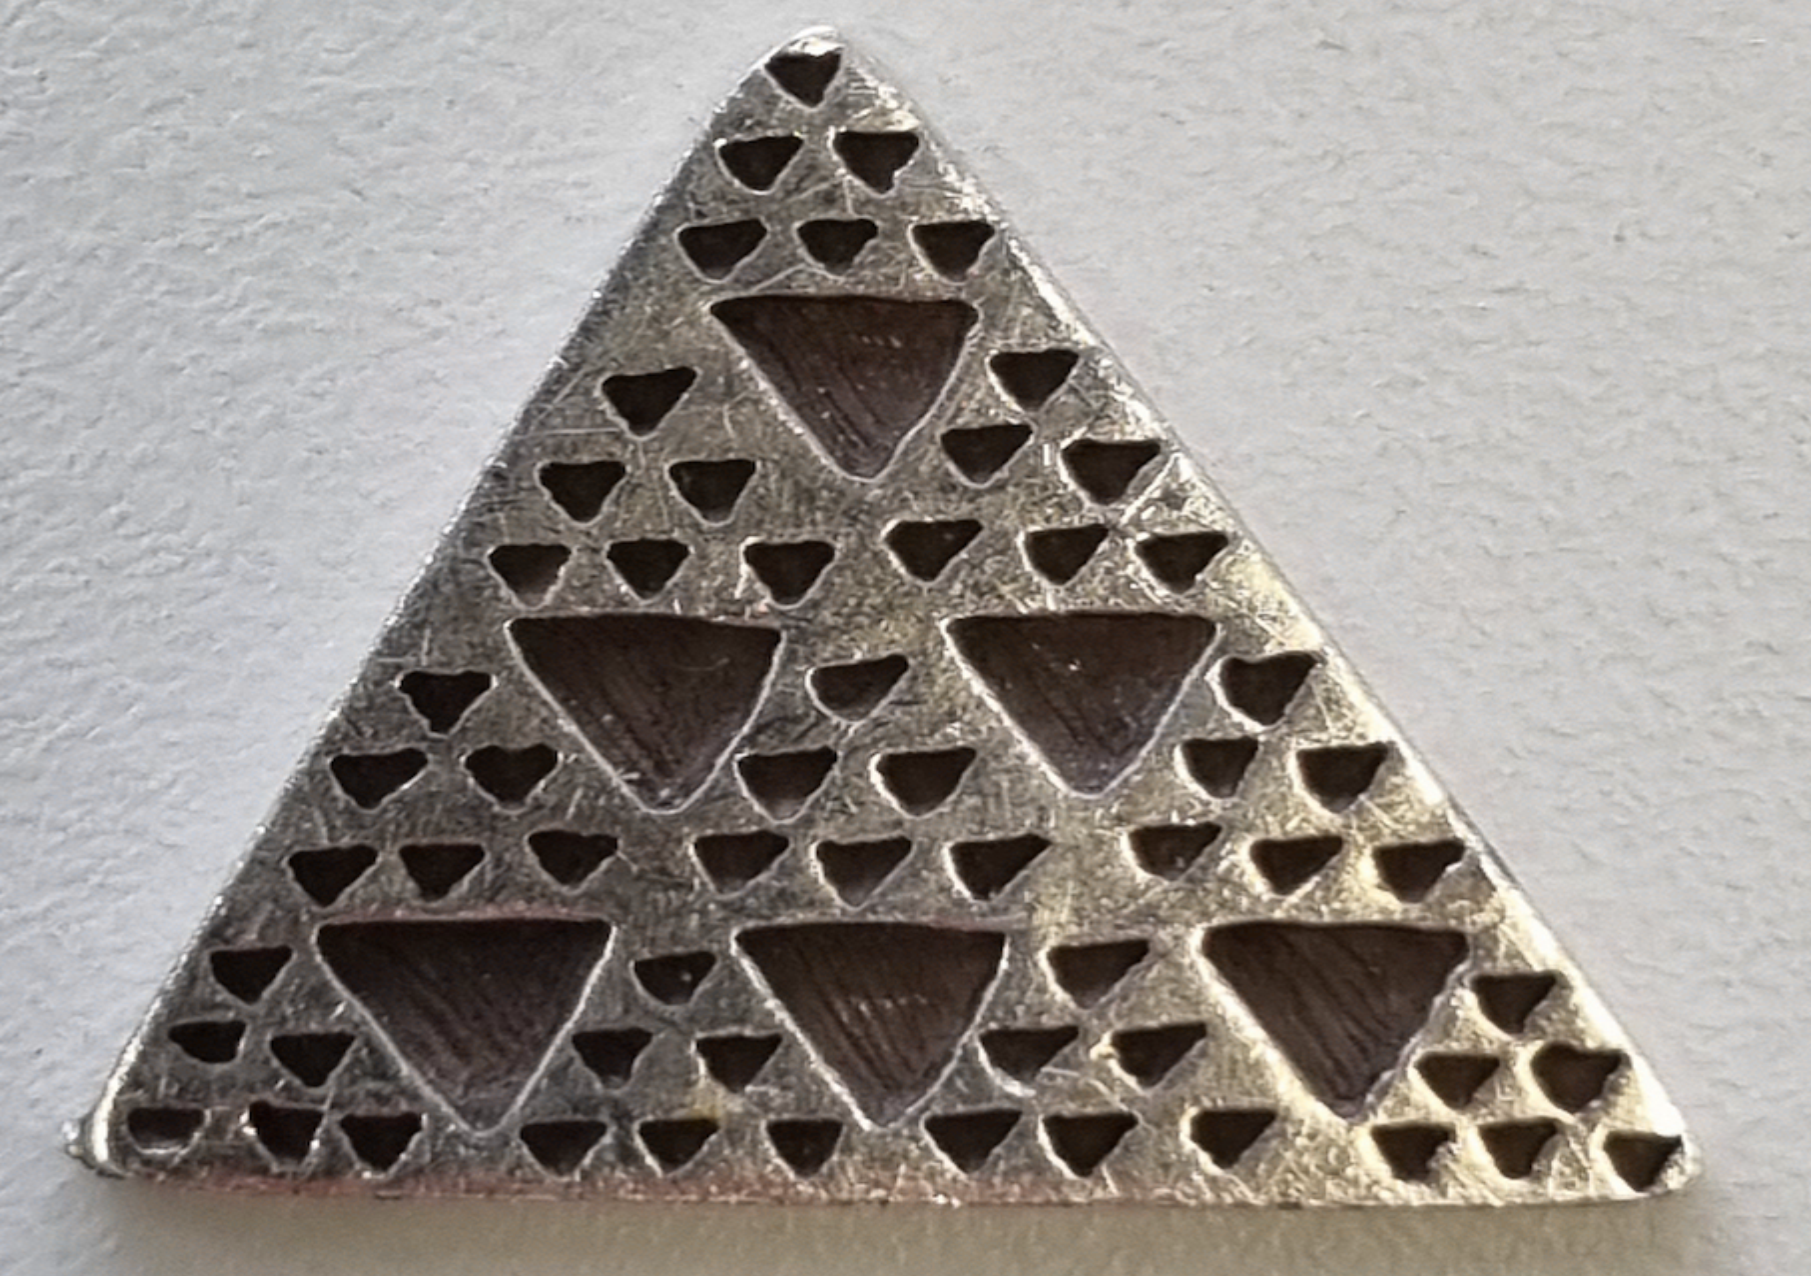
\includegraphics[width=80mm, height=60mm] {triangle.png}    
\end{figure}

 
 
 
 \vskip 6mm

 \noindent {\bf 3.}   Demuestra que si $R_j$ es una colección de rectángulos centrados en el origen del plano $\mathbb R^2$ con la propiedad de que $\displaystyle \lim_{j\to\infty} \mbox{diag}(R_j)= 0,$ entonces, si $1<p<\infty$ y $f\in L^p(\mathbb R^2)$ se tiene
 $$
 \lim_{j\to\infty}\frac 1{|R_j|}\int_{R_j} f(x-y)\, dy = f(x), \quad \mbox{a.e. }  x.
 $$
 {\it Indicación}: Pruébalo primero para funciones continuas con soporte compacto y luego demuestra (y usa a continuación) que el operador maximal, $M_s$, sobre ese tipo de rectángulos está acotado por la composición de dos operadores maximales unidimensionales de Hardy-Littlewood $M_1, \, M_2$ de la forma
 $$
 M_1f(x_1,x_2)=\sup_{h>0}\; \frac1{2h}\int_{-h}^{h}|f(x_1-t,x_2)|\, dt.
 $$
 (De forma similar se define $M_2$.)
   
\vskip 6mm
\hrule
\vskip 5mm

\noindent {\bf SOL.:} 
 
 \end{document}